\documentclass[a4paper]{scrreprt}
%\documentclass[a4paper]{report}

% Uncomment to optimize for double-sided printing.
% \KOMAoptions{twoside}

% Set binding correction manually, if known.
% \KOMAoptions{BCOR=2cm}

% Localization options
\usepackage[english]{babel}
\usepackage[T1]{fontenc}
\usepackage[utf8]{inputenc}

% Enhanced verbatim sections. We're mainly interested in
% \verbatiminput though.
\usepackage{verbatim}

% PDF-compatible landscape mode.
% Makes PDF viewers show the page rotated by 90°.
\usepackage{pdflscape}

% Advanced tables
\usepackage{tabu}
\usepackage{longtable}

% Fancy tablerules
\usepackage{booktabs}

% Graphics
\usepackage{graphicx}

\usepackage{float}

% Current time
\usepackage[useregional=numeric]{datetime2}

% Float barriers.
% Automatically add a FloatBarrier to each \section
\usepackage[section]{placeins}

% Custom header and footer
\usepackage{fancyhdr}
\setlength{\headheight}{15.2pt}
\pagestyle{fancyplain}

\usepackage{geometry}
\usepackage{layout}

% Math tools
\usepackage{mathtools}
% Math symbols
\usepackage{amsmath,amsfonts,amssymb}

\fancyhf{}
% Chapter header on non-plain pages only.
\lhead{\fancyplain{} {\leftmark}}
% Footer must contain print date. Ugly, but IPA requirement.
\lfoot{\printdate}
% Print date left and page count right was the thing which looked the
% most balanced.
\rfoot{\thepage}
% 
% Source code & highlighting
\usepackage{listings}

% Convenience commands
\newcommand{\mailsubject}{2407 - Computernetze - Practical exercise 2}
\newcommand{\maillink}[1]{\href{mailto:#1?subject=\mailsubject}
                               {#1}}

% Should use this command wherever the print date is mentioned.
\newcommand{\printdate}{\today}

\subject{2407 - Computernetze}
\title{Practical exercise 3}

\author{Michael Senn \maillink{michael.senn@students.unibe.ch}}

\date{\printdate}

% Needs to be the last command in the preamble, for one reason or
% another. 
\usepackage{hyperref}


\begin{document}
\maketitle

% \tableofcontents

\chapter{IPSec VPN}

For this exercise we have set up an IPSec VPN between the two routers R1 and
R2, therefore allowing eg transparently encrypted communication between VM1 and
VM2 over an (imaginary) insecure network.

\section{Router configuration}

\subsection{Access lists}

In order to determine which traffic will be encrypted, ACLs were used. In this
case, ACLs are a list of source/destination tuples, against which traffic is
matched. If they do match one of the ACL's conditions, it will be encrypted.

In this case, we have decided to only encrypt traffic which is between VM1 and
VM2. If desired, it would be easy to change this ACL to eg encrypt all traffic
between the two subnets the VMs reside in. One such possible configuration is
included in the snippet below, albeit commented out. It should be noted that
ACLs use wildcard masks rather than subnet masks - wildcard masks being the
inverse of their corresponding subnet mask.

\begin{lstlisting}[caption=Router 1]
conf t

! access-list 100 permit ip 10.0.1.0 0.0.0.255 10.0.2.0 0.0.0.255
access-list 100 permit ip host 10.0.1.2 host 10.0.2.2

exit
\end{lstlisting}

\begin{lstlisting}[caption=Router 2]
conf t

! access-list 100 permit ip 10.0.2.0 0.0.0.255 10.0.1.0 0.0.0.255
access-list 100 permit ip host 10.0.2.2 host 10.0.1.2

exit
\end{lstlisting}

\subsection{Cryptography settings}

Next, we configured several things
\begin{description}
	\item[IPSec Transform sets] Here we defined with which algorithm
		traffic is processed. The two IPsec peers have to have at least
		one set of operations in common.
	\item[Crypto maps] Here we defined the IPSec peer of a given router, as
		well as which transform set to use.
	\item[ISAKMP policy] Here we defined the mechanism of the security key
		exchange. In our case, we decided to use a pre-shared key for
		simplicity.
\end{description}

\begin{lstlisting}[caption=Router 1]
conf t

crypto ipsec transform-set ex3 esp-des esp-md5-hmac

crypto map ex3 10 ipsec-isakmp
match address 100
set peer 10.0.100.2
set transform-set ex3
exit

crypto isakmp policy 1
hash md5
authentication pre-share
exit

crypto isakmp key 0 secretkey address 10.0.100.2 255.255.255.255

exit
\end{lstlisting}

\begin{lstlisting}[caption=Router 2]
conf t

crypto ipsec transform-set ex3 esp-des esp-md5-hmac

crypto map ex3 10 ipsec-isakmp
match address 100
set peer 10.0.100.1
set transform-set ex3
exit

crypto isakmp policy 1
hash md5
authentication pre-share
exit

crypto isakmp key 0 secretkey address 10.0.100.1 255.255.255.255

exit
\end{lstlisting}

\subsection{Interface configuration}

Lastly, the defined crypto maps had to be applied to the interfaces between
which the tunnel was going to be established.

\begin{lstlisting}[caption=Router 1]
conf t

interface fastethernet 0/1
crypto map ex3
exit

exit
\end{lstlisting}

\begin{lstlisting}[caption=Router 2]
conf t

interface fastethernet 0/0
crypto map ex3
exit

exit
\end{lstlisting}

\section{Results}

In order to comfortably test whether traffic between machines was encrypted, we
used \texttt{netcat}, which allows to open a basic TCP server on one machine,
and send arbitrary data to it from another. In our case we used it to send
plaintext messages, which could be read on the other end.

In addition, we used Wireshark to capture traffic on the two hubs between R2
and R1/R3 respectively.

\subsection{VM2 - VM3}

As there was no IPSec tunnel set up between the two Routers R2 and R3, this
traffic was not encrypted. This can be clearly seen in various ways.

\begin{itemize}
\item Source and destination IP are IPs of VM2 / VM3.
\item The protocol used atop of IP is TCP.
\item The sent message body can be seen in the payload.
\end{itemize}

\subsection{VM2 - VM1}

As an IPsec tunnel was set up, traffic beteween R2 and R1 will be encrypted.
This can be seen in several ways:

\begin{itemize}
\item Source and destination IP are IPs of the routers, due to them tunneling
	packets.
\item The protocol used atop of IP is ESP.
\item The sent message body can not be seen in the payload.
\end{itemize}

\subsection{Screenshots VM2 - VM3}

\begin{figure}[H]
    \centering
    \textbf{Netcat server on VM3}\par\medskip
    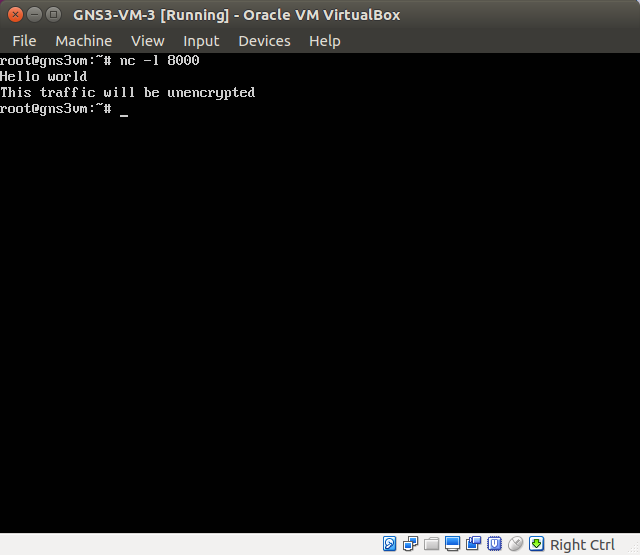
\includegraphics[width=0.9\textwidth]{resources/nc_vm3.png}
\end{figure}

\begin{figure}[H]
    \centering
    \textbf{Netcat client on VM2 to VM3}\par\medskip
    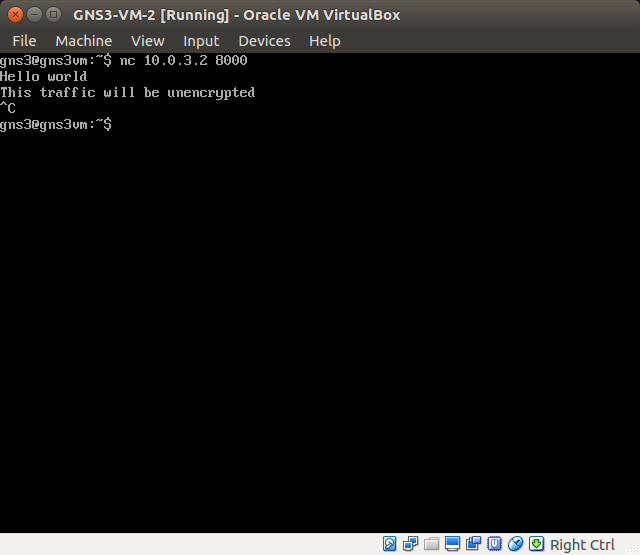
\includegraphics[width=0.9\textwidth]{resources/nc_vm2_to_vm3.png}
\end{figure}

\begin{figure}[H]
    \centering
    \textbf{Non-encrypted traffic on hub}\par\medskip
    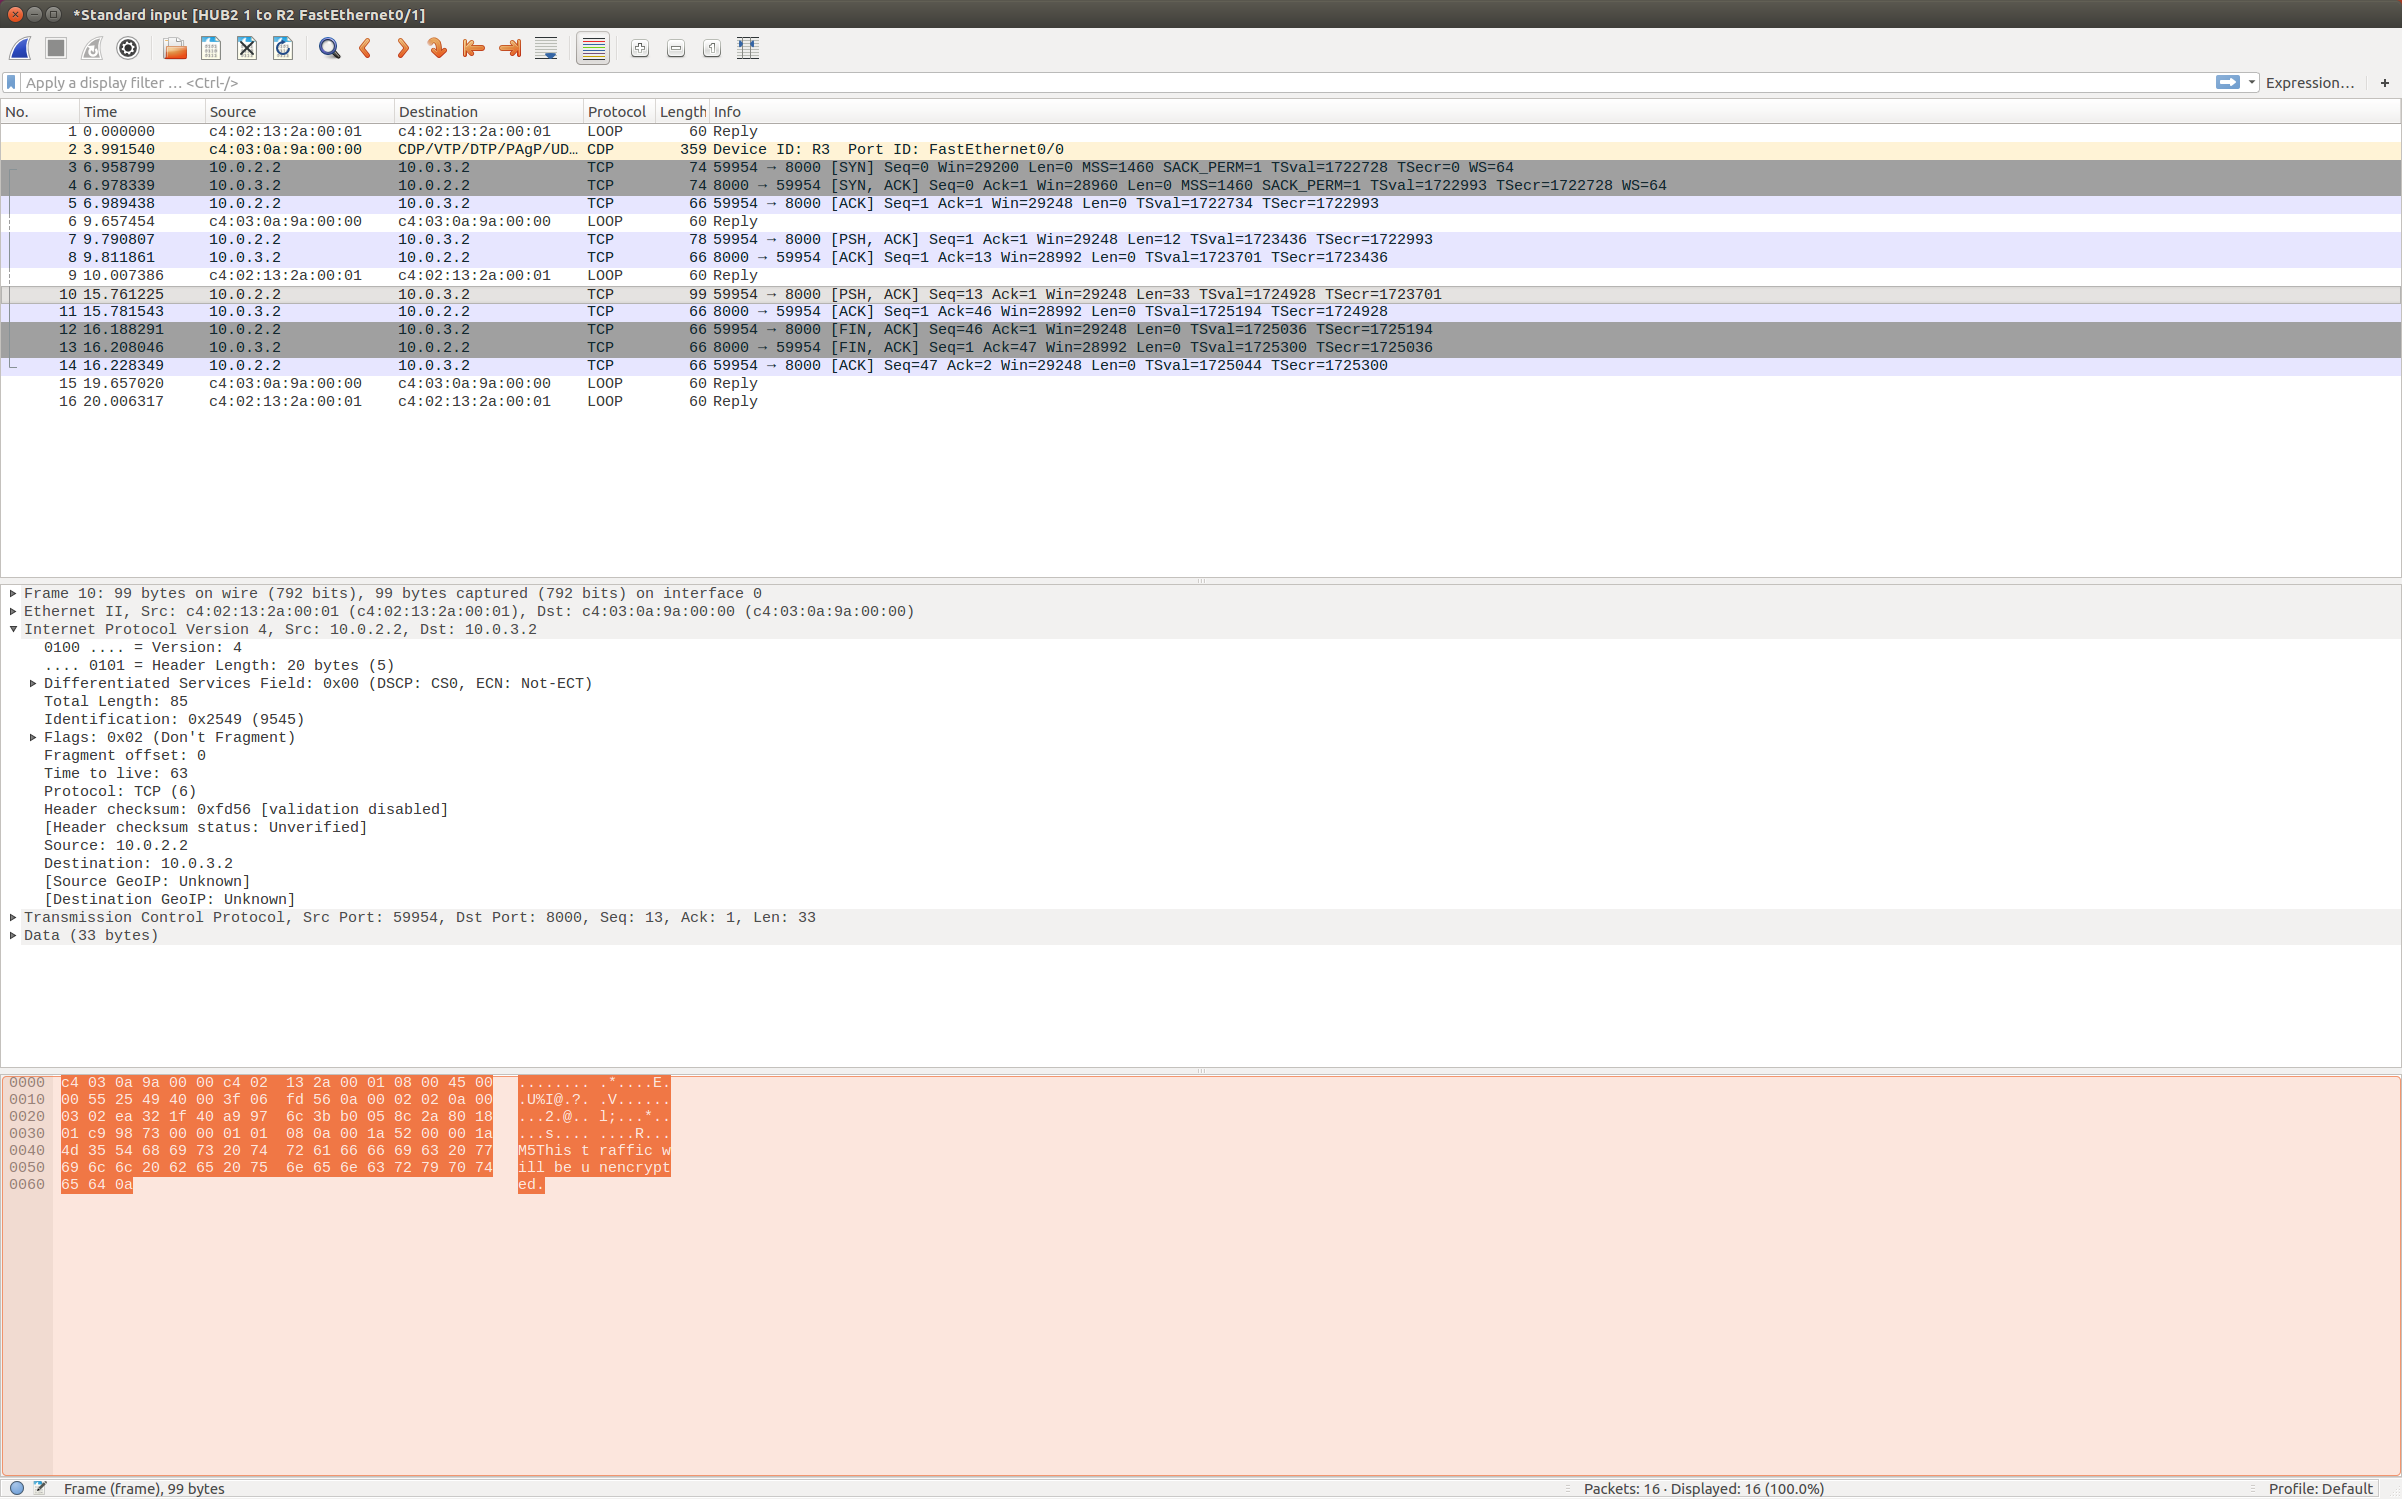
\includegraphics[width=0.9\textwidth]{resources/wireshark_hub2_to_r2.png}
\end{figure}

\subsection{Screenshots VM2 - VM1}

\begin{figure}[H]
    \centering
    \textbf{Netcat server on VM1}\par\medskip
    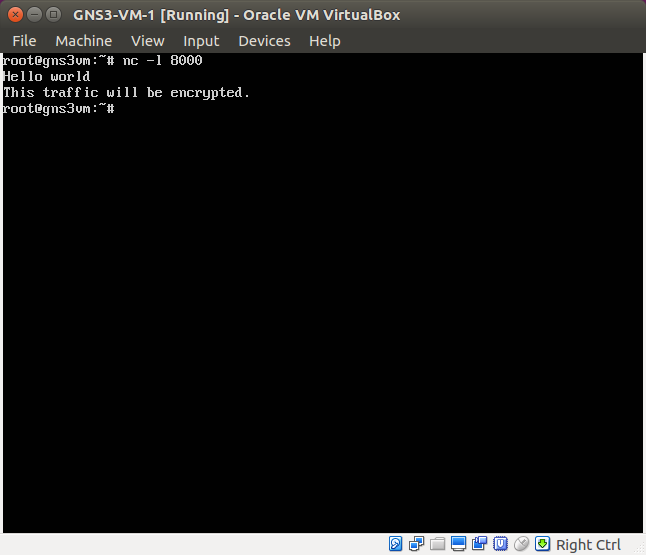
\includegraphics[width=0.9\textwidth]{resources/nc_vm1.png}
\end{figure}

\begin{figure}[H]
    \centering
    \textbf{Netcat client on VM2 to VM1}\par\medskip
    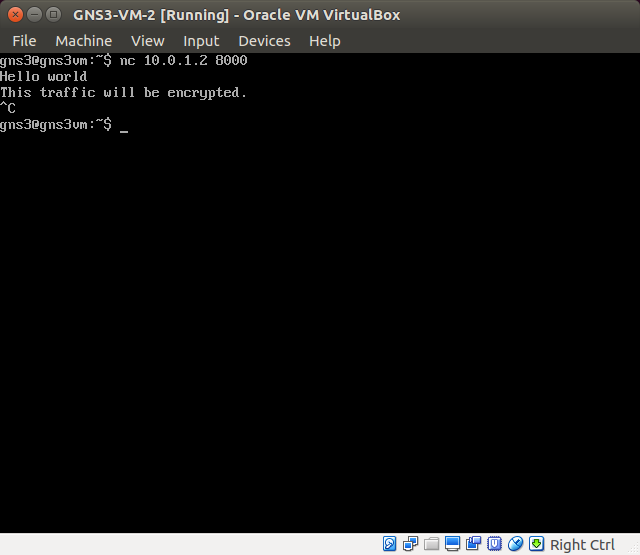
\includegraphics[width=0.9\textwidth]{resources/nc_vm2_to_vm1.png}
\end{figure}

\begin{figure}[H]
    \centering
    \textbf{Encrypted traffic on hub}\par\medskip
    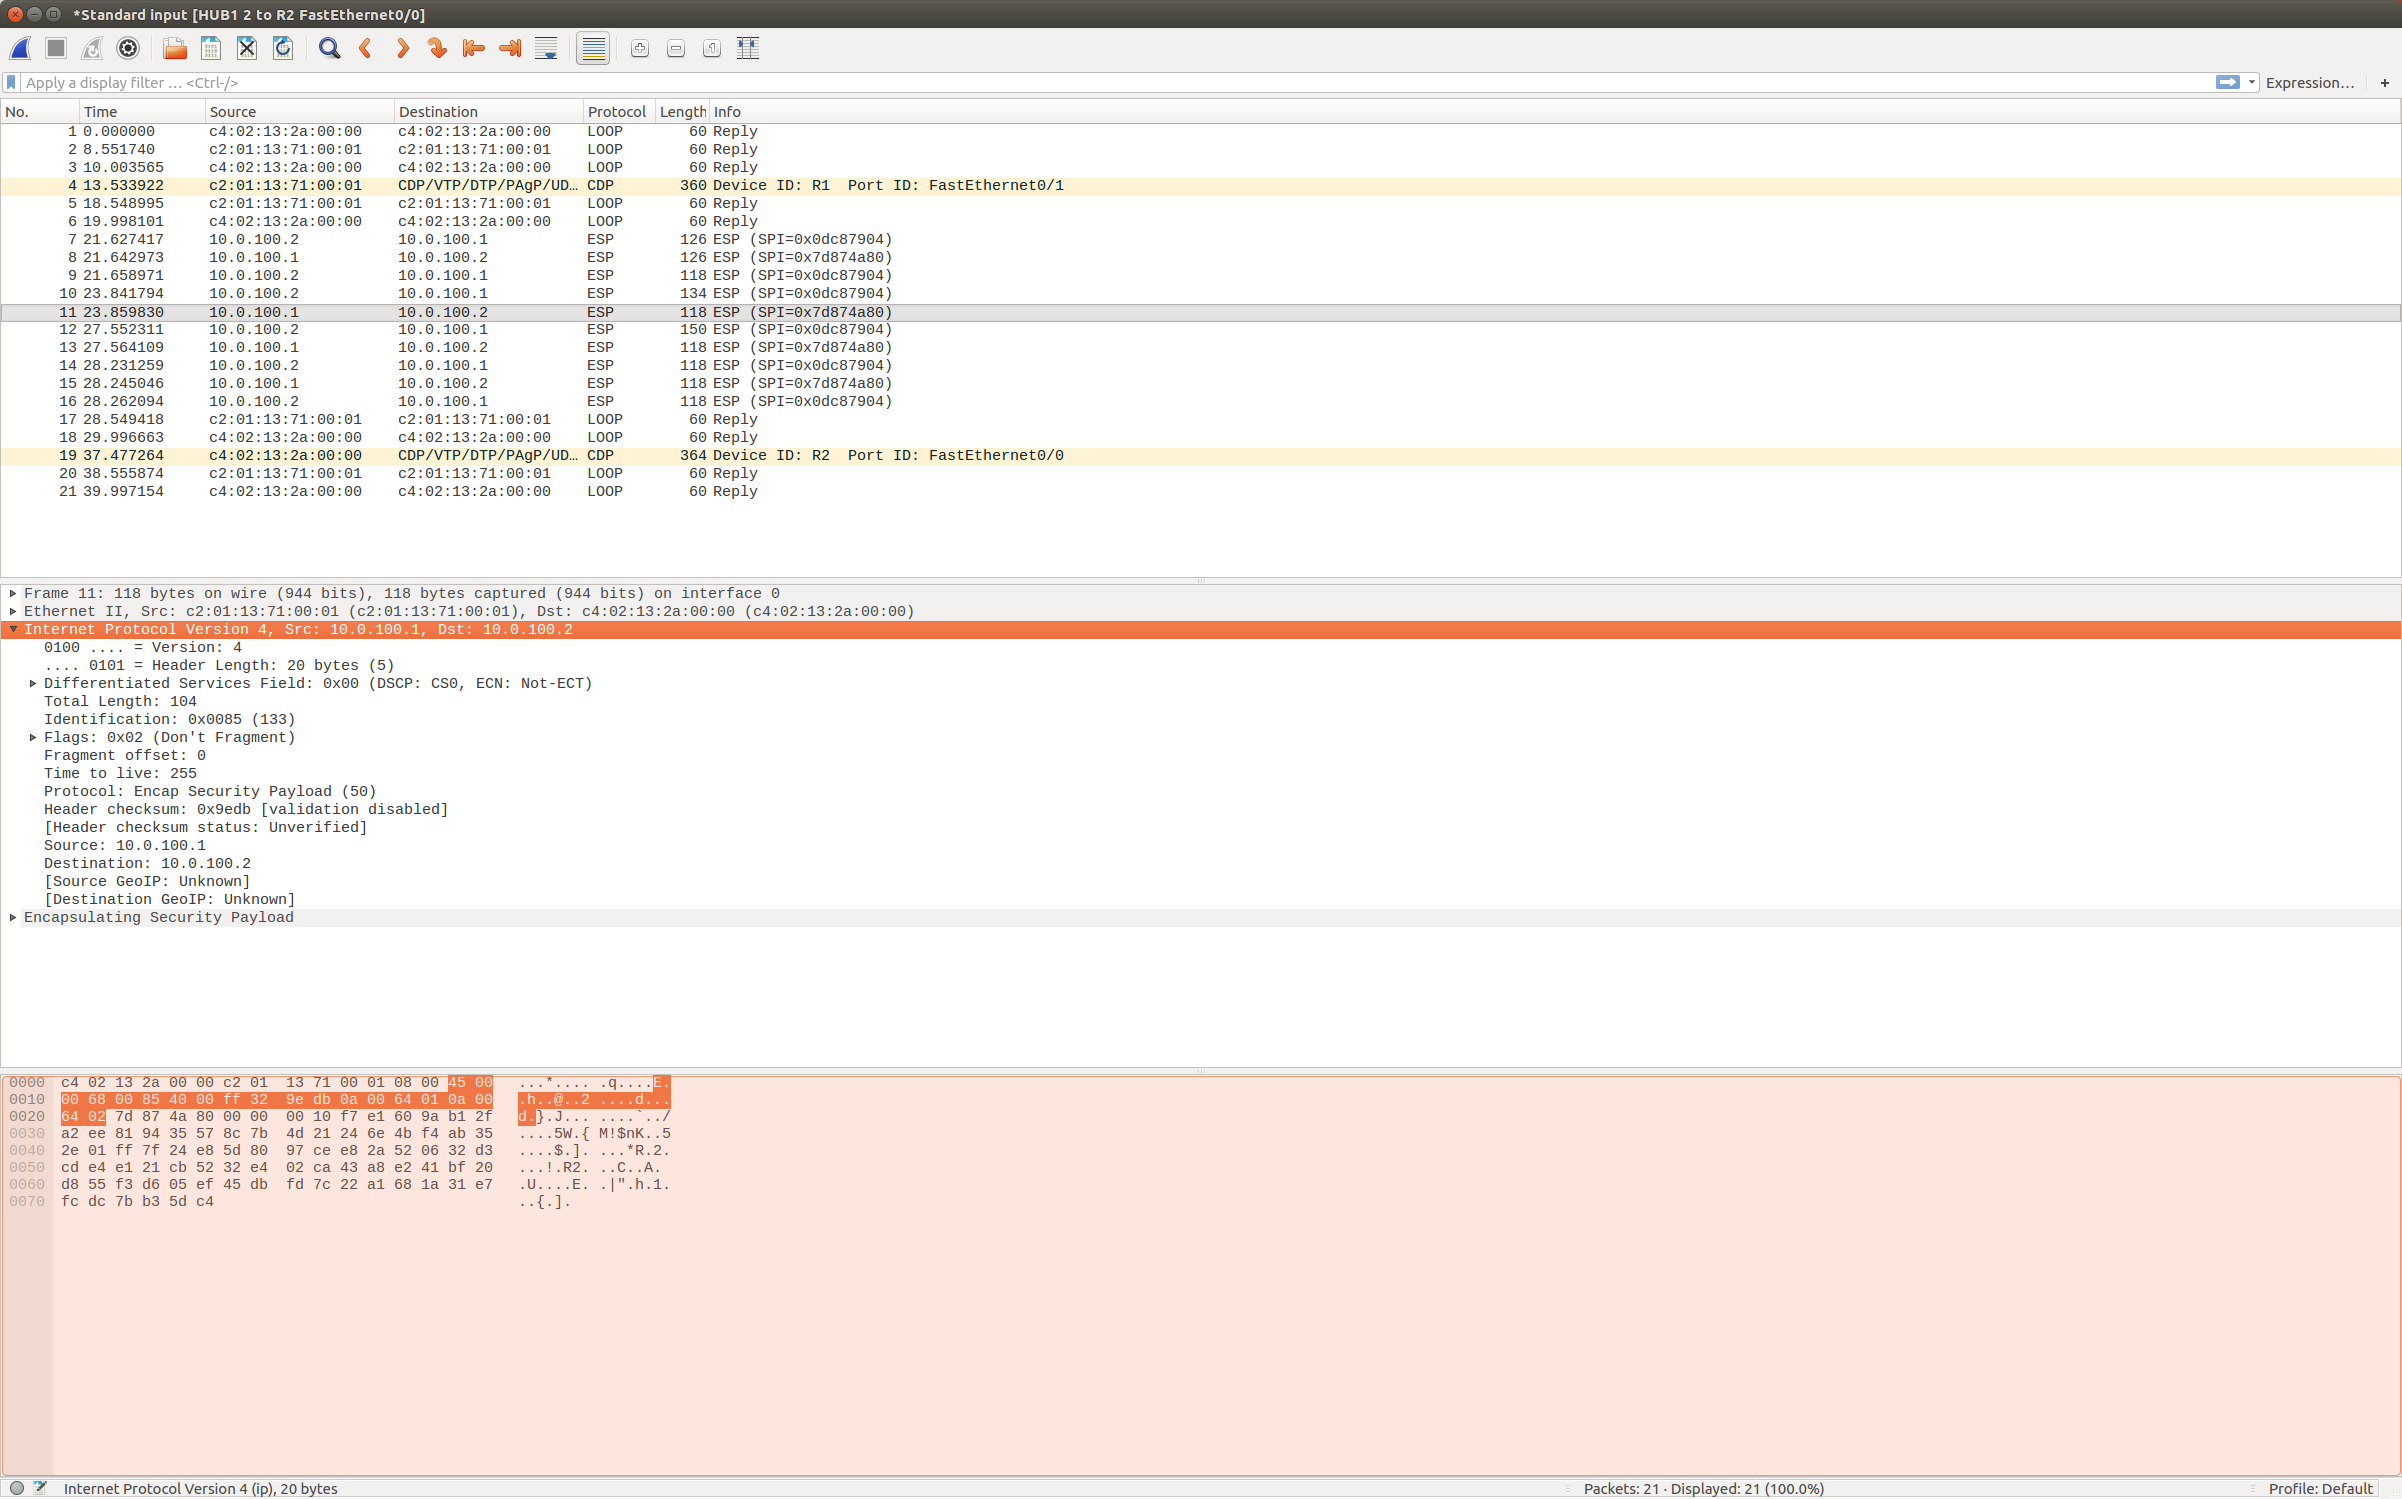
\includegraphics[width=0.9\textwidth]{resources/wireshark_hub1_to_r2.png}
\end{figure}


\end{document}
